\section{Espansione}

\subsection{Aggiunta tripletta model-view-controller} \label{sec:aggiuntamvc}
Per inserire una tripletta MVC i passaggi verranno elencati prima nello specifico di ogni componente ed infine verrà esplicitato come collegare correttamente ogni componente. Per maggiori informazioni sulla struttura del codice fare riferimento a \S{}\ref{sec:cartelle-src}

\subsubsection{Aggiunta model}
Per aggiungere un nuovo model bisogna creare una nuova classe all'interno della cartella "model" che erediti dalla classe "\textit{QObject}". Se esso deve implementare il pattern singleton fare riferimento a \S{}\ref{sec:singleton-python}. La nuova componente del modello dovrà avere un segnale al suo interno per comunicare i cambiamenti del suo stato, il segnale è una variabile di classe istanziata con il seguente codice: \texttt{Sg\_model\_changed = Signal()} e ad ogni cambiamento di stato del modello deve essere segnalato emettendo un segnale così: \texttt{self.Sg\_model\_changed.emit()}.


\subsubsection{Aggiunta view}
Per aggiungere una nuova parte della view bisogna creare una nuova classe all'interno della cartella "view". Se si tratta di una view da rappresentare nella stessa finestra delle altre essa dovrà essere istanziata nel costruttore della classe \textit{"MainWidget"} e sempre nel costruttore essere aggiunto ai widget della classe. Il codice per l'aggiunta è il seguente: \newline{} \centerline{ \texttt{self.swidget.addWidget(new\_widget)}.}
Questa aggiunta viene mostrata con una sottolineatura nella seguente immagine:
\begin{figure}[H]
    \centering
    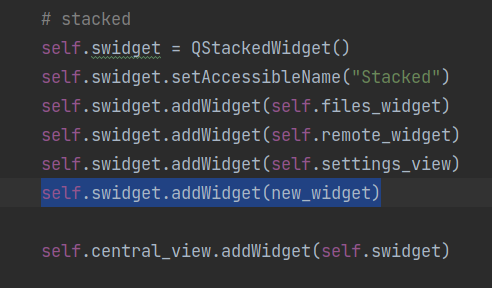
\includegraphics[scale = 0.75]{components/img/codice-nuova-view-su-main-view.png}
    \caption{Codice per inserimento nuova view nella main view}
    \label{fig:Codice per inserimento nuova view nella main view}
\end{figure}
La view deve inoltre esporre un metodo per ricevere segnali dal modello, questo lo si realizza marcando il metodo in questione con il decorator "\textit{@Slot()}".
\subsubsection{Aggiunta controller}
Per aggiungere una nuova parte del controller bisogna creare una nuova classe all'interno della cartella "controllers". Il controller deve inoltre esporre un metodo per ricevere segnali dalla vista, questo lo si realizza marcando il metodo in questione con il decorator "\textit{@Slot()}".

\subsubsection{Collegamento componenti}
Dopo aver creato le strutture di ogni componente della nuova tripletta MVC il controller viene utilizzato per collegare il tutto. 
Si deve quindi collegare il segnale emanato dalla nuova vista ad ogni cambiamento al metodo con decorator @Slot() precedentemente creato nel controller e il segnale emanato dal model ad ogni cambiamento al metodo con decorator @Slot() precedentemente creato nella vista. Il collegamento avviene nel costruttore del controller utilizzando la sintassi mostrata nella seguente immagine:
\begin{figure}[H]
    \centering
    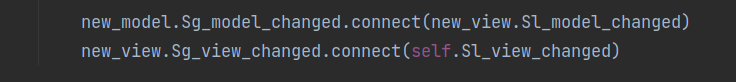
\includegraphics[scale = 0.50]{components/img/collegamento-segnali-mvc.png}
    \caption{Collegamento componenti MVC}
    \label{fig:Collegamento componenti MVC}
\end{figure}
Il metodo connect può essere solo invocato su segnali e come argomento devono avere il riferimento al metodo con decorator @Slot().

\subsection{Aggiunta nuovi test}
\subsubsection{Creazione del file di test}
La creazione del nuovo file di test deve avvenire nella corretta folder seguendo la struttura definita a \S{}\ref{sec:cartelle-tests}. 
Il nome del file deve seguire la seguente sintassi: \newline{} \centerline{\textbf{nome\_test.py}}
La sintassi è esplicata nella seguente tabella:
{
    \setlength{\freewidth}{\dimexpr\textwidth-1\tabcolsep}
    \renewcommand{\arraystretch}{1.5}
    \setlength{\aboverulesep}{0pt}
    \setlength{\belowrulesep}{0pt}
    \rowcolors{2}{AzzurroGruppo!10}{white}
    \begin{longtable}{L{.20\freewidth} L{.80\freewidth}}
        \rowcolor{AzzurroGruppo!30}
        \textbf{Parola chiave} & \textbf{Descrizione}\\
        \toprule
        \endhead
        \textbf{nome} & Il nome scelto per identificare la classe testata. Di norma viene utilizzato il nome della classe testata.\\
        \textbf{\_} & Separatore da utilizzare tra il nome della classe testata e la parola test.\\
        \textbf{test} & Parola chiave di utilizzo obbligatorio per permettere l'esecuzione automatica del test. \\
        \bottomrule
        \hiderowcolors
        \caption{Descrizione della sintassi utilizzata per creare file di test}
    \end{longtable}
}
Se la parola "test" non dovesse essere trovata nel nome del file o non dovesse essere separata correttamente tramite il carattere "\_" il test non verrà eseguito automaticamente all'esecuzione del comando indicato a \S{} \ref{sec:unittest}.
\subsubsection{Creazione della classe di test}
Il nome della nuova classe di test segue la seguente sintassi: \newline{} \centerline{\textbf{NomeTest.py}}
La sintassi è esplicata nella seguente tabella:
{
    \setlength{\freewidth}{\dimexpr\textwidth-1\tabcolsep}
    \renewcommand{\arraystretch}{1.5}
    \setlength{\aboverulesep}{0pt}
    \setlength{\belowrulesep}{0pt}
    \rowcolors{2}{AzzurroGruppo!10}{white}
    \begin{longtable}{L{.20\freewidth} L{.80\freewidth}}
        \rowcolor{AzzurroGruppo!30}
        \textbf{Parola chiave} & \textbf{Descrizione}\\
        \toprule
        \endhead
        \textbf{Nome} & Il nome scelto per identificare la classe testata. Di norma viene utilizzato il nome della classe testata.\\
        \textbf{Test} & Parola chiave utilizzata per esplicitare la funzione di test della classe. Il suo uso non è obbligatorio ma permette una maggiore chiarezza nel codice. \\
        \bottomrule
        \hiderowcolors
        \caption{Descrizione della sintassi utilizzata per creare classi di test}
    \end{longtable}
}
Questa nuova classe deve ereditare dalla classe base di ogni test "\textit{DefaultCode}" ed implementare correttamente i metodi "SetUp" e "TearDown" come mostrato nella seguente tabella:
{
    \setlength{\freewidth}{\dimexpr\textwidth-1\tabcolsep}
    \renewcommand{\arraystretch}{1.5}
    \setlength{\aboverulesep}{0pt}
    \setlength{\belowrulesep}{0pt}
    \rowcolors{2}{AzzurroGruppo!10}{white}
    \begin{longtable}{L{.20\freewidth} L{.80\freewidth}}
        \rowcolor{AzzurroGruppo!30}
        \textbf{Parola chiave} & \textbf{Descrizione}\\
        \toprule
        \endhead
        \textbf{SetUp} & Metodo eseguito automaticamente prima di ogni test. Deve sempre, come prima istruzione, chiamare il metodo SetUp della classe base DefaultCode.\\
        \textbf{TearDown} & Metodo eseguito automaticamente dopo ogni test. Deve sempre, come prima istruzione, chiamare il metodo TearDown della classe base DefaultCode.\\
        \bottomrule
        \hiderowcolors
        \caption{Descrizione della corretta implementazione dei metodi SetUp e TearDown}
    \end{longtable}
}

\subsubsection{Creazione dei nuovi metodi di test}
Il nome dei nuovi metodi segue la seguente sintassi:\newline{}\centerline{\textbf{test\_nome}}
Dove:
{
    \setlength{\freewidth}{\dimexpr\textwidth-1\tabcolsep}
    \renewcommand{\arraystretch}{1.5}
    \setlength{\aboverulesep}{0pt}
    \setlength{\belowrulesep}{0pt}
    \rowcolors{2}{AzzurroGruppo!10}{white}
    \begin{longtable}{L{.20\freewidth} L{.80\freewidth}}
        \rowcolor{AzzurroGruppo!30}
        \textbf{Parola chiave} & \textbf{Descrizione}\\
        \toprule
        \endhead
       \textbf{test} & Parola chiave che deve obbligatoriamente essere presente all'inizio del nome del metodo per poter essere eseguito automaticamente.\\
        \textbf{\_} & Separatore da utilizzare tra le parole.\\
        \textbf{nome} & Il nome della funzionalità testata.\\
        \bottomrule
        \hiderowcolors
        \caption{Descrizione della corretta denominazione di nuovi metodi di test}
    \end{longtable}
}
La logica base di ogni test si compone in:
\begin{itemize}
    \item Chiamata del metodo interessato;
    \item Controllo dei risultati ottenuti dal metodo.
\end{itemize}
Il controllo dei risultati si esegue con il seguente codice:\newline{} \centerline{\texttt{result = classe.metodo()}}\newline{}\centerline{\texttt{self.assertEqual(result, risultato\_previsto)}}\newline{}
La sintassi del controllo dei risultati è meglio descritta nella seguente tabella:
{
    \setlength{\freewidth}{\dimexpr\textwidth-1\tabcolsep}
    \renewcommand{\arraystretch}{1.5}
    \setlength{\aboverulesep}{0pt}
    \setlength{\belowrulesep}{0pt}
    \rowcolors{2}{AzzurroGruppo!10}{white}
    \begin{longtable}{L{.30\freewidth} L{.70\freewidth}}
        \rowcolor{AzzurroGruppo!30}
        \textbf{Parola chiave} & \textbf{Descrizione}\\
        \toprule
        \endhead
        \textbf{self.assertEqual} & Metodo ereditato dalla classe base DefaultCode che lo eredita a sua volta da unittest.TestCase. Questo metodo confronta i due argomenti a lui dati e nel caso in cui non siano uguali fa fallire il test.\\
        \textbf{result} & Il risultato del metodo da noi chiamato. \\
        \textbf{risultato\_previsto} & Il risultato che ci aspettiamo il metodo restituisca.\\
        \bottomrule
        \hiderowcolors
        \caption{Descrizione della logica di base dei metodi di test.}
    \end{longtable}
}
